\documentclass[border=10pt]{standalone}

\usepackage{tikz}
\usepackage{tikzsymbols}
\usetikzlibrary{calc,patterns,shapes.geometric}

\def\centerarc[#1](#2)(#3:#4:#5){\draw[#1] ($(#2)+({#5*cos(#3)},{#5*sin(#3)})$) arc (#3:#4:#5);}

\begin{document}
	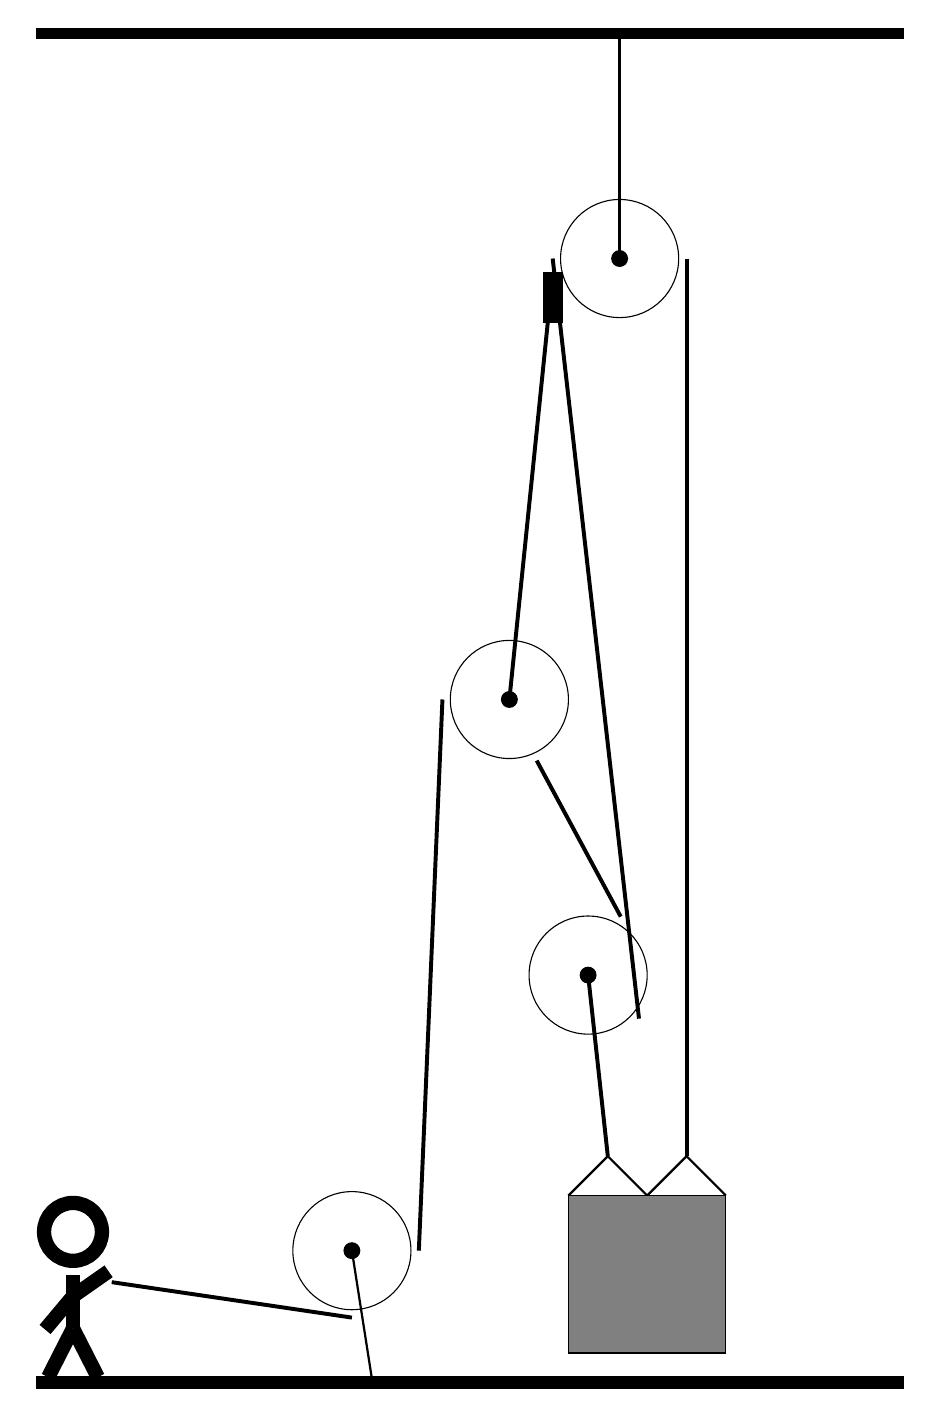
\begin{tikzpicture}
		%%%%% START %%%%%
		\draw[fill=black] (-6, 14) rectangle (5, 14.125);
		
		\draw (0, 5.6) circle (0.75);
		\draw[fill=black] (0, 5.6) circle (0.1);
		
		\draw (1, 2.1) circle (0.75);
		\draw[fill=black] (1, 2.1) circle (0.1);
		
		\draw (1.4, 11.2) circle (0.75);
		\draw[fill=black] (1.4, 11.2) circle (0.1);
		\draw[very thick] (1.4, 11.2) -- (1.4, 14);
		
		\draw (-2, -1.4) circle (0.75);
		\draw[fill=black] (-2, -1.4) circle (0.1);
		\draw[thick] (-2, -1.4) -- (-1.75, -3);
		
		
		\draw[thick]  (0.75, -0.7) -- (1.25, -0.2) -- (1.75, -0.7) -- (2.25, -0.2) -- (2.75, -0.7);
		\draw[fill=black!50] (0.75, -0.7) rectangle (2.75, -2.7);
		\draw[line width=0.5mm] (-5.05, -1.8) -- (-2, -2.25);
		\centerarc[line width=0.5mm](-2, -1.4)(270:360:0.85);
		\draw[line width=0.5mm] (-1.15, -1.4) -- (-0.85, 5.6);
		\draw[line width=0.5mm] (0, 5.6) -- (0.55, 11.0);
		\draw[line width=0.5mm, fill=black](0.45, 10.4) rectangle (0.65, 11.0);
		\centerarc[line width=0.5mm](0, 5.6)(-20:180:0.85);
		\draw[line width=0.5mm] (0.347, 4.824) -- (1.414, 2.842);
		\centerarc[line width=0.5mm](1, 2.1)(160:380:0.85);
		\draw[line width=0.5mm] (1.646, 1.547) -- (0.55, 11.2);
		\draw[line width=0.5mm](1, 2.1) -- (1.25, -0.2);
		\centerarc[line width=0.5mm](1.4, 11.2)(0:180:0.85);
		\draw[line width=0.5mm] (2.25, 11.2) -- (2.25, -0.2);
		
		\node at (-5.5, -1.9) {\Strichmaxerl[10][50][35]};
		
		\draw[fill=black] (-6, -3) rectangle (5, -3.15);
		%%%%% END %%%%%
	\end{tikzpicture}
\end{document}